%! suppress = SentenceEndWithCapital
%! suppress = TooLargeSection
%! suppress = FigureNotReferenced
%! suppress = FileNotFound
\documentclass[12pt,twoside]{report}
\usepackage{float}
\usepackage{textcomp}
\usepackage{siunitx}
%%%%%%%%%%%%%%%%%%%%%%%%%%%%%%%%%%%%%%%%%%%%%%%%%%%%%%%%%%%%%%%%%%%%%%%%%%%%%

% Definitions for the title page
% Edit these to provide the correct information
% e.g. \newcommand{\reportauthor}{Timothy Kimber}

\newcommand{\reporttitle}{ABM in Finance - Climate Impact}
\newcommand{\reportauthor}{Hanzhe HUANG}
\newcommand{\supervisor}{Prof. Luk, Wayne}
\newcommand{\degreetype}{M.Sc Computing}

%%%%%%%%%%%%%%%%%%%%%%%%%%%%%%%%%%%%%%%%%%%%%%%%%%%%%%%%%%%%%%%%%%%%%%%%%%%%%

% load some definitions and default packagesload some definitions and default packagesload some definitions and
% default packages
%! suppress = DiscouragedUseOfDef
%! suppress = DiscouragedUeOfDef
%%%%%%%%%%%%%%%%%%%%%%%%%%%%%%%%%%%%%%%%%
% University Assignment Title Page 
% LaTeX Template
% Version 1.0 (27/12/12)
%
% This template has been downloaded from:
% http://www.LaTeXTemplates.com
%
% Original author:
% WikiBooks (http://en.wikibooks.org/wiki/LaTeX/Title_Creation)
%
% License:
% CC BY-NC-SA 3.0 (http://creativecommons.org/licenses/by-nc-sa/3.0/)
% 
%
%%%%%%%%%%%%%%%%%%%%%%%%%%%%%%%%%%%%%%%%%
%----------------------------------------------------------------------------------------
%	PACKAGES AND OTHER DOCUMENT CONFIGURATIONS
%----------------------------------------------------------------------------------------
\usepackage[a4paper,hmargin=2.8cm,vmargin=2.0cm,includeheadfoot]{geometry}
\usepackage{textpos}
\usepackage{natbib} % for bibliography
\usepackage{tabularx,longtable,multirow,subfigure,caption}%hangcaption
% \usepackage{fncylab} %formatting of labels
\usepackage{fancyhdr} % page layout
\usepackage{url} % URLs
\usepackage[english]{babel}
\usepackage{amsmath}
\usepackage{graphicx}
% \usepackage{dsfont}
\usepackage{epstopdf} % automatically replace .eps with .pdf in graphics
\usepackage{backref} % needed for citations
\usepackage{array}
% \usepackage{latexsym}
\usepackage[pdftex,pagebackref,hypertexnames=false,colorlinks]{hyperref} % provide links in pdf

% \usepackage{url}

\hypersetup{pdftitle={},
  pdfsubject={}, 
  pdfauthor={},
  pdfkeywords={}, 
  pdfstartview=FitH,
  pdfpagemode={UseOutlines},% None, FullScreen, UseOutlines
  bookmarksnumbered=true, bookmarksopen=true, colorlinks,
    citecolor=black,%
    filecolor=black,%
    linkcolor=black,%
    urlcolor=black}

\usepackage[all]{hypcap}


%\usepackage{color}
%\usepackage[tight,ugly]{units}
%\usepackage{float}
%\usepackage{tcolorbox}
%\usepackage[colorinlistoftodos]{todonotes}
% \usepackage{ntheorem}
% \theoremstyle{break}
% \newtheorem{lemma}{Lemma}
% \newtheorem{theorem}{Theorem}
% \newtheorem{remark}{Remark}
% \newtheorem{definition}{Definition}
% \newtheorem{proof}{Proof}


%%% Default fonts
\renewcommand*{\rmdefault}{bch}
\renewcommand*{\ttdefault}{cmtt}



%%% Default settings (page layout)
\setlength{\parindent}{0em}  % indentation of paragraph

\setlength{\headheight}{14.5pt}
\pagestyle{fancy}
\renewcommand{\chaptermark}[1]{\markboth{\chaptername\ \thechapter.\ #1}{}} 

\fancyfoot[ER,OL]{\sffamily\textbf{\thepage}}%Page no. in the left on odd pages and on right on even pages
\fancyfoot[OC,EC]{\sffamily }
\renewcommand{\headrulewidth}{0.1pt}
\renewcommand{\footrulewidth}{0.1pt}
\captionsetup{margin=10pt,font=small,labelfont=bf}


%--- chapter heading

\def\@makechapterhead#1{%
  \vspace*{10\p@}%
  {\parindent \z@ \raggedright \sffamily
    \interlinepenalty\@M
    \Huge\bfseries \thechapter \space\space #1\par\nobreak
    \vskip 30\p@
  }}

%---chapter heading for \chapter*  
\def\@makeschapterhead#1{%
  \vspace*{10\p@}%
  {\parindent \z@ \raggedright
    \sffamily
    \interlinepenalty\@M
    \Huge \bfseries  #1\par\nobreak
    \vskip 30\p@
  }}

\allowdisplaybreaks

% load some macros
% Here, you can define your own macros. Some examples are given below.

\newcommand{\R}[0]{\mathds{R}} % real numbers
\newcommand{\Z}[0]{\mathds{Z}} % integers
\newcommand{\N}[0]{\mathds{N}} % natural numbers
\newcommand{\C}[0]{\mathds{C}} % complex numbers
\renewcommand{\vec}[1]{{\boldsymbol{{#1}}}} % vector
\newcommand{\mat}[1]{{\boldsymbol{{#1}}}} % matrix


\date{June 2021}

\begin{document}

% load title page
	% Last modification: 2015-08-17 (Marc Deisenroth)
\begin{titlepage}

\newcommand{\HRule}{\rule{\linewidth}{0.5mm}} % Defines a new command for the horizontal lines, change thickness here


%----------------------------------------------------------------------------------------
%	LOGO SECTION
%----------------------------------------------------------------------------------------


\includegraphics[width = 4cm]{./figures/imperial}\\[0.5cm] 

\center % Center remainder of the page

%----------------------------------------------------------------------------------------
%	HEADING SECTIONS
%----------------------------------------------------------------------------------------

\textsc{\Large Imperial College London}\\[0.5cm] 
\textsc{\large Department of Computing}\\[0.5cm] 

%----------------------------------------------------------------------------------------
%	TITLE SECTION
%----------------------------------------------------------------------------------------

\HRule \\[0.4cm]
{ \huge \bfseries \reporttitle}\\ % Title of your document
\HRule \\[1.5cm]
 
%----------------------------------------------------------------------------------------
%	AUTHOR SECTION
%----------------------------------------------------------------------------------------

\begin{minipage}{0.4\textwidth}
\begin{flushleft} \large
\emph{Author:}\\
\reportauthor % Your name
\end{flushleft}
\end{minipage}
~
\begin{minipage}{0.4\textwidth}
\begin{flushright} \large
\emph{Supervisor:} \\
\supervisor % Supervisor's Name
\end{flushright}
\end{minipage}\\[4cm]


%----------------------------------------------------------------------------------------
%	FOOTER & DATE SECTION
%----------------------------------------------------------------------------------------
\vfill % Fill the rest of the page with whitespace
Submitted in partial fulfillment of the requirements for the MSc degree in
\degreetype~of Imperial College London\\[0.5cm]

\makeatletter
\@date 
\makeatother


\end{titlepage}



% page numbering etc.
	\pagenumbering{roman}
	\clearpage{\pagestyle{empty}\cleardoublepage}
	\setcounter{page}{1}
	\pagestyle{fancy}

%%%%%%%%%%%%%%%%%%%%%%%%%%%%%%%%%%%%
% 	\begin{abstract}
% 		test
%
% 	\end{abstract}
	
	% \cleardoublepage
	% \clearpage
%%%%%%%%%%%%%%%%%%%%%%%%%%%%%%%%%%%%
% 	\section*{Acknowledgments}
% 	Comment this out if not needed.\\
	
	
	% \clearpage{\pagestyle{empty}\cleardoublepage}

%%%%%%%%%%%%%%%%%%%%%%%%%%%%%%%%%%%%
%--- table of contents
	\fancyhead[RE,LO]{\sffamily {Table of Contents}}
	\tableofcontents
	\clearpage%{\pagestyle{empty}\cleardoublepage}
	\pagenumbering{arabic}
	\setcounter{page}{1}
	\fancyhead[LE,RO]{\slshape \rightmark}
	\fancyhead[LO,RE]{\slshape \leftmark}

%%%%%%%%%%%%%%%%%%%%%%%%%%%%%%%%%%%%
	
	
	\chapter{Introduction}\label{ch:introduction}
	2015 marks a historical year on human history with the Paris Agreement was commonly agreed by the vast majority
	of country or region entities after long conditional pledges.
	While governments agreed to pursue a well below 2\textcelsius, widely interpreted as 1.5\textcelsius, the
	pathway and mitigation goal set at the time was found to be not as sufficient as retrodicted with the long-term
	ambition~\cite{Schleussner2016}.
	At least 7.6\% annual reduction in global greenhouse emission was expected up to 2030 and
	onwards~\cite{UNEP2019, Eric2020}.
	Furthermore, global emission has barely dropped by 8\% annually since the pandemic with devastating impact on
	travelling and manufacturing.
	As the world recovers from pandemic, burden on emission control would be considerably heavy~\cite{Eric2020,
		dafnomilis2020}.
	A synthetic green recovery became a consensus.\\
	
	Developing a policymaking model has been drawing scientists' attention for over 30 years and, this is a
	challenging task due to the nature of this complex System-of-System problem.
	A series of heterogeneous and partially independent groups or individuals interact with each
	other~\cite{GERST201362}.
	Interaction among government policy, industry-specific strategy, economic response, and eventually the impact on
	climate is at the core of understanding the environmental crisis and setting off to make difference.
	This project aims to apply the agent-based modelling approach to simulate this interaction within the
	human-environment system under different scenarios.
	More specifically, under what circumstance will the goal of Paris Agreement be reached or not, and what are the
	corresponding performance is of interest.


%%%%%%%%%%%%%%%%%%%%%%%%%%%%%%%%%%%%
	
	%! suppress = TooLargeSection
	
	
	\chapter{Literature Review}\label{ch:literature-review}
	%---------------%
	
	
	\section{Agent Based Modelling approach}\label{sec:agent-based-modelling-approach}
	Agent based modeling is an uprising approach that simulates the interaction
	among multiple (groups) of intelligent agents within a system.
	The very basic concept behind this approach is so-called cellular automation
	which was first devised in the Conway's Game of Life in 1970~\cite{Conway1970}.
	With simple rules and random seeds, the individual cells evolves into surprising
	functional patterns.
	One fascinating feature of this modelling technique is the undecidability.
	That is, given a starting point, there is no algorithm that could give a definite
	prediction on how will this system evolves~\cite{golomb1983elwyn},
	This is what distinguish the ABM method from other popular equation based
	models or machine-learning solutions where the system is simplified into a series of
	homogeneous equations with invisible interaction~\cite{sun2005survey,ABMEqu1998}.\\
	
	State-of-art agent based model works inherits the core principle from the Conway's
	Game of Life and mainly consists of three key elements\cite{macal2014introductory}:
	\begin{enumerate}
		\item \textbf{Agents}\\
		Each agent can be seen as a dispersive and smart individual that is of
		their own attributes and methods defining the behaviour.
		\item \textbf{Agent Relationships}\\
		Agents are expected to interact with each other.
		An underlying topology defining the range and method of this interaction
		is expected.
		Similar to individuals in real world, the relationship and interaction
		could be either global or local, i.e.limited knowledge.
		\item \textbf{Environment}\\
		Agents are supposed to live in an environment and, inevitably, interact
		with it.
	\end{enumerate}
	Rational and representative definition of these elements lays the foundation
	of a contributing agent based model.
	\clearpage
	%---------------%
	
	
	\section{Apply ABM on Climate Issue}\label{sec:climate-impact-on-economic-metrics}
	With the capability of the micro-scope simulation, ABM has been utilized on investigating a
	range of
	specific
	scope relating to the climate policy, such as emission reduction, energy portfolio and electric vehicle
	transition~\cite{Castro2020, MUELLER20091072}.\\
	
	Firstly, Gerst, Wang, Roventini, et al.~\cite{GERST201362} presented a model that simulates the trend of GDP,
	energy use, carbon emissions and energy price under the customer appliance sector.
	Their work attempts to describe the interaction with a so-called two-level ENGAGE model, where the level 1
	represents the international negotiation entities such as nations or global organizations.
	Level 2 represents the domestic economy-energy portfolio including firms, households and national/regional climate
	mitigation policies.
	The outcome from domestic activity would be the basis for the negotiator's action, figure\ref{fig:ENGAGE} shows the
	structure.
	\begin{figure}[htb]
		\centering
		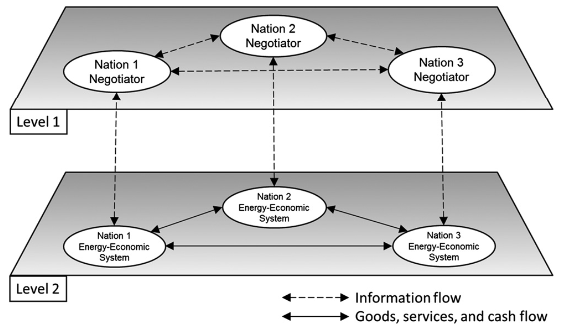
\includegraphics[width = 0.6\linewidth]{./figures/ENGAGE}
		\caption{Two-Level ENGAGE Model\cite{GERST201362}}
		\label{fig:ENGAGE}
	\end{figure}
	
	In brief, energy technology firms evolves along either carbon-heavy, carbon-light or green path, and
	corresponding three types of energy productions are of different prices that varies with technology productivity,
	demand and policy affects.
	To-business suppliers and to-customer appliance manufactures uses energy and make production.
	They invest certain amount of their profit on R\&D and thus improve their products' efficiency and reduce price.
	Households in this model works as labour force on these firms.
	Their wages would be used to purchase and use a certain amount of appliances that could either be kept or replaced
	according to households' individual evaluation.
	Domestic authorities enforce carbon tax punishing high emission practices in order to reduce the overall emission
	induced by energy production, manufacturing and the use of appliances.
	The carbon tax collected could be either rebated to households, incentive manufacturers' R\&D or invested on
	green energy.
	Reference scenario is set to be no carbon tax in place.
	\\
	
	Over 100 years of iteration, it was proved that all three types of tax usage could lead to significant drop on
	the energy intensity per unit of GDP, comparing with no carbon tax reference.
	However, in terms of emission metrics, investing on green-energy technology is the only possible solution leading
	to satisfying emission drop, by more than 50\%, and increment of carbon-free energy share.
	Although household rebates and manufacturing R\&D incentives would contribute to a lower peak emission, they both
	end up with no difference at the end of 21st century comparing with no carbon tax at all.
	Interestingly, under the green-energy investment scenario, the energy intensity of consumer appliances were even
	higher than the reference with a 50\% more total energy use and nearly 100\% GDP growth in the end.
	Interestingly, under the green-energy investment scenario, total energy use is 50\% more than other cases
	while the total emission 60\%less.
	Nearly 75\% GDP growth is also achieved.
	This shows the ultimacy of developing carbon-free energy.
	\begin{figure}[htb]
		\centering
		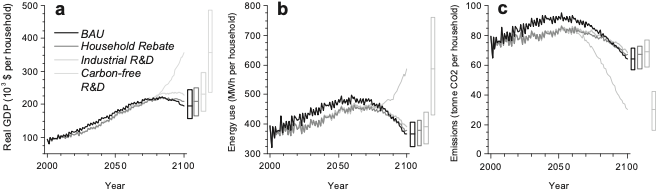
\includegraphics[width = 1\linewidth]{./figures/ENGAGE_Result}
		\caption{Predicted annual (a)GDP, (b)energy use, (c)emissions per household\cite{GERST201362}}
		\label{fig:ENGAGE_Result}
	\end{figure}
	
	While the development on green energy became a consensus, scientists narrowed down their focus to specific
	aspects.
	For example, transportation acts as a key role on climate issue with the non-negligible amount of emissions
	induced, especially in urban area.
	Scientists attempted to investigate the effect that a variety of traffic policies has on the primary emission
	due to urban commuting~\cite{hofer2018large}.
	In this research, a full scale urban network of an Austrian city was replicated with real roadmap and commuting
	options.
	Each agent acts as a citizen that travels around with individual from/to and preference on the means of
	transportation.
	Along with a reference, several scenarios, such as promoting private electric vehicles, replacing old vehicles,
	develop public transports and expand current roads to reduce congestion were taken into consideration.\\
	
	With a realistic validation in place, the model shows that replacing private fuel vehicles with EV is of highest
	potential for emission reduction overall, given the fact that the percentage of private car ownership is
	relatively high in europe.
	Public transport is another promising solution.
	In addition to the emission drop, it also contributes to less congestion in peak hours, as a result of lower
	traffic flow.
	However, this may require a delicate design on the public network, and a combination with the solution to "last
	mile".
	Note that, although this model only focuses on primary emission of transportation itself and neglects the issue
	related to energy source and some secondary effects, the approaches demonstrated here could still be a quantitative
	method on such aspect-specific studies.\\
	\clearpage
	
	While the potential of EV is seen by public, question arising is how to promote EVs to the broad public.
	Efforts were made on incorporating the individual behaviour under different EV incentives\cite{MUELLER20091072}.
	Here comes the advantage of ABM, where each individual could act heterogeneously and forms a general observation.
	In this work, a population of individuals were initialised with current car ownerships and sociodemographic frames,
	e.g.\ age, household structure and income level.
	These are the preconditions for further vehicle purchase or replacement that would be considered when modeling
	the behaviour.
	Above this, researchers involved outcome from behavioural-economic theory and decision-making characteristics.
	These features contribute to a more realistic and intuitive individual agents.\\
	
	Result shows that the feebate policy has a positive effect by encouraging people to adapt or select those
	vehicles with lower emission, either with smaller engine or with hybrid/EV drive.
	The class of vehicles roughly remains stable, as this is decided by the mandatory quota on passenger/goods
	capacity, range, etc.
	Furthermore, the feebate would not cause the rebound effect, i.e.\ incentive on greener vehicles would not lead
	to a growth on overall quantity of vehicles.
	However, all these evaluations is based on acceptance and transparency on the policy itself.
	Note that This research is based on real statistics of technical data and price of individual on sale vehicles,
	which makes it much easier to understand with strong robustness.
	
	%---------------%
	
	
	\section{Macroscopic Research}\label{sec:marco-scopic-climate-and-finance-research}
	Other than the bottom-up micro-simulation described above, an ABM could also utilize macroscopic parameters drawn
	from statistics on economy, climate and other study areas\cite{Castro2020}.
	As soon as the environment became a focus of human being, a growing body of empirical studies has been
	evaluating the inter-relationship between climate observations and socioeconomic behaviours.\\
	
	Firstly, climate change was proved to have direct and significant impact on primary industry, such as
	agricultural output\cite{moore2017new} and electricity consumption\cite{wenz2017north}.
	Non-catastrophic warming has a diverged impact with respect to the countries' baseline
	temperature\cite{burke2015global}.
	Slight rise on annual average temperature may help those cooler countries, e.g.\ european countries, to increase
	the GDP growth,    yet tropical countries suffers extra loss from every extra step on warming.
	This trend does not vary with the level of development or the accumulation of social and technical capital.
	However, in the worst cases, global GDP may see a nearly 50\% loss by 2100 and severe
	polarization\cite{burke2015global}.
	More optimistic studies supports around 3.5--4\textcelsius temperature rise on global annual average with 7--14\%
	drop on global output\cite{howard2017few, kalkuhl2020impact}.
	All these researches did not take secondary damage from more frequent extreme weathers and social impact into
	consideration.
	Presumably severer situation is possible.\\
	\clearpage
	Recent study draws attention to the day-to-day temperature variation\cite{Day2Day}.
	Strong negative correlation between the monthly standard deviation of temperature and the percentage loss of GDP
	growth rate was proved.
	One extra degree of temperature variation would result in 5\% slower GDP growth in global average.
	Developed regions with higher level of base variation may be more capable of adapting the variation, others may
	have lost nearly 10\% annual GDP growth over the past 40 years.
	National coordination across different regions does help to, yet not fundamentally, mitigate the difference.
	What frustrating is that this phenomenon is independent with the global warming and acts on its own.
	This new impact channel definitely worth more concern.
	
	\begin{figure}[htb]
		\begin{minipage}[t]{0.51\linewidth}
			\centering
			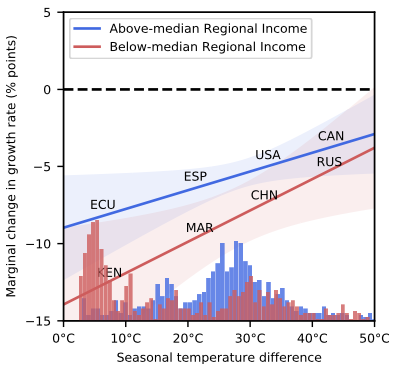
\includegraphics[width=1\linewidth]{./figures/D2D-national}
			% \caption{a}
		\end{minipage}%
		\begin{minipage}[t]{0.49\linewidth}
			\centering
			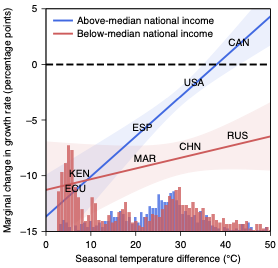
\includegraphics[width=1\linewidth]{./figures/D2D-regional}
			% \caption{b}
		\end{minipage}
		\caption{The change in regional growth rates per extra degree of day-to-day temperature variability estimated
		separately for \texttt{region} \& \texttt{countries} with above- and below-median income per
		capita\cite{Day2Day}}
		\label{fig:NeoLayer}
	\end{figure}

%%%%%%%%%%%%%%%%%%%%%%%%%%%%%%%%%%%%
	
	
	\chapter{Technical Progress}\label{ch:technicall-progress}
	This project implements the development kit fromSimudyne\textregistered \space technology.
	Simudyne\textregistered \space is the one of the in-trend enterprise-level supplier that provides agent-based
	modeling solution to large financial institutions\cite{Simudyne}.
	Robustness and reliability is widely proven.
	The product is a Java SDK package that supports ABM in Java environment.
	At this beginning stage, a simple agent-based model was build as a walk-through practice.
	This model attempts to show the initial purchasing and replacing of passenger vehicles.\\
	
	Firstly, the total number ov fuel vehicles and EVs are set to be global accumulator.
	Then, Agents of \texttt{Brand} and \texttt{Households} groups were set.
	Households were initialised a budget over a certain range and no vehicle ownership.
	Conventional vehicles are preferred at initial stage, and household would purchase one if the price is accepted.
	Once a household owns a fuel vehicle, they monitor the driving cost of EV and replace with EV if the cost drops
	to certain level.
	The brand produces conventional or electric vehicles.
	Initially, the EV is of higher price and lower cost comparing with conventional vehicles.
	At each time frame, the brand would evolve both types and reduces price and the unit driving cost.
	R\&D progress on EV was assumed to be more aggressive, leading to quicker drops on both price and unit cost than
	the other.
	The updated information would be broadcasted to all customers, who makes their own decision and send the
	sell/buy EV/conventional decision back to brand.
	Finally, the brand sums up these decisions and update the global accumulator.
	All these assumptions were fulfilled with simple dummy numbers.\\
	\clearpage
	
	In this scenario, it is expected that conventional vehicles would dominate the market as all households with
	sufficient budget would buy one.
	Later on, the EV price quickly drops, and those households with lower budget would then go for an EV.
	At the end of the day, significant saving on EV usage encourages the fuel-vehicle-owning switches to EV.
	Actual implementation is validated with expected performance
	
	\begin{figure}[h]
		\centering
		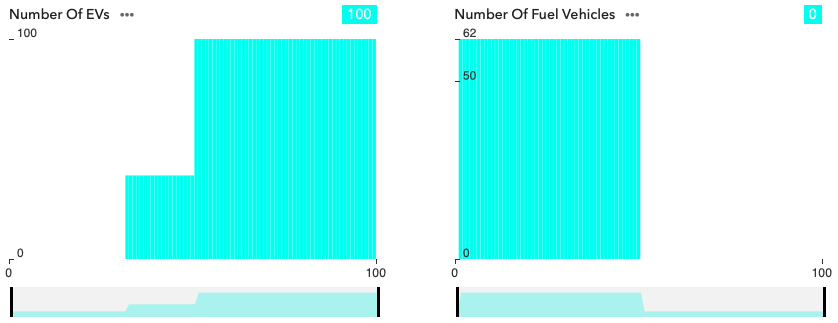
\includegraphics[width = 1\linewidth]{./figures/dummy}
		\caption{Dummy model result with Simudyne}
		\label{fig:dummy}
	\end{figure}


%%%%%%%%%%%%%%%%%%%%%%%%%%%%%%%%%%%%
	
	
	\chapter{Further Plan}\label{ch:further-plan}
	This project aims to build a model with some high-level parameters describing economy and climate issues.
	Main reason is that, a comprehensive model could be built with a relatively small amount of data by this
	approach, comparing with the specific-focus model described in previous section where much more detail statistics
	is necessary.
	As recommended, the ABM model should be built in an iterative process~\cite{macal2014introductory}.
	Additional features, rules and agents groups should be added step by step and gradually forms a complete model.
	In general, the 3-step technical plan for this project would be as following:
	\begin{enumerate}
		\item Build global model with average parameters.
		\item Introduce regional and periodic specifications
		\item Finalising project with refining, tuning and possibly accelerating
	\end{enumerate}
	Throughout this project, tracking changes and documentation of the data source is of vital importance when
	validating the finished product.
	Addition effort is expected.


%%%%%%%%%%%%%%%%%%%%%%%%%%%%%%%%%%%%
	
	
	% \chapter{Conclusion}\label{ch:conclusion}
	%
	% test~\cite{Dij1,Dij2,Dij3,Astar}


%% bibliography
	\bibliographystyle{unsrt}
	\bibliography{ref}


\end{document}
